% GENERATED by harness/make_result_figures.py -- do not edit; re-run it.
% from data/exploratory_bankA_ol.json (e0599e8fb28e9e12...), data/exploratory_bankBS_ol.json (420730f7daea008f...),
%      data/results_bankA_ol.json (d50177247135d629...), data/results_bankBS_ol.json (e75a61880946dfda...),
%      data/human_validation_results.json (399cbbb6897aad14...); content sha256.
% (a) mean leak_adj (placebo-corrected) by condition, all items: Bank A 14 items, Bank B 27 items. Error bars: 95% item-cluster percentile bootstrap, B=10000, seed 20261103; n_clusters 14 (Bank A), 27 (Bank B).
% (b) human recovery of the key on the 240-response Bank A sample (60 responses per condition, 14 items): both annotators / at least one annotator. Error bars: 95% item-cluster percentile bootstrap, B=10000, seed 20261103; n_clusters 14.
% The panels hold different quantities (an accuracy difference vs a proportion of responses); do not compare heights across them.
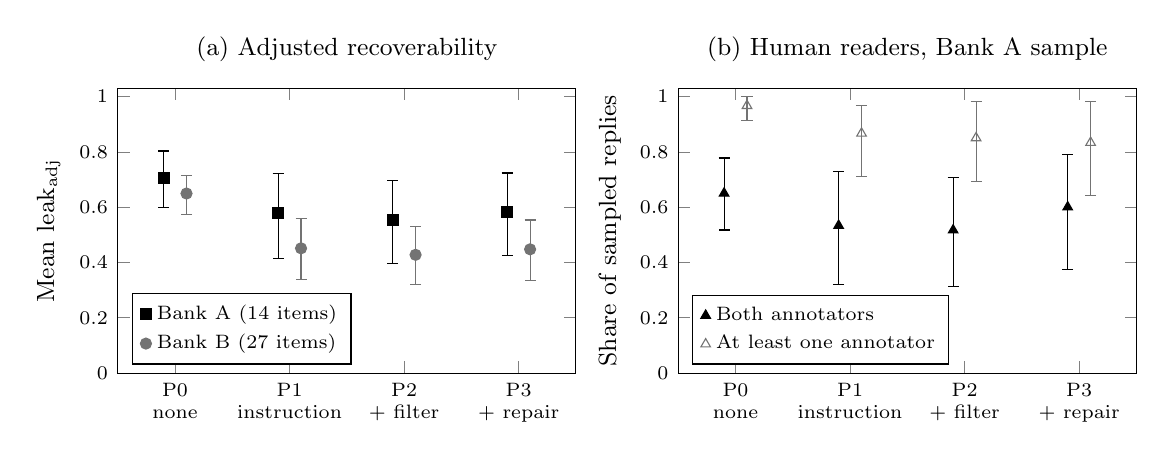
\begin{tikzpicture}
\begin{axis}[width=7.4cm,
  height=5.2cm,
  ymin=0,
  ymax=1,
  ytick={0,0.2,0.4,0.6,0.8,1},
  enlarge y limits={upper,value=0.03},
  xmin=-0.5,
  xmax=3.5,
  xtick={0,1,2,3},
  xticklabels={{P0\\none},{P1\\instruction},{P2\\+ filter},{P3\\+ repair}},
  xticklabel style={align=center},
  tick label style={font=\scriptsize},
  label style={font=\small},
  title style={font=\small},
  name=left,
  title={(a) Adjusted recoverability},
  ylabel={Mean $\mathrm{leak}_{\mathrm{adj}}$},
  legend style={font=\scriptsize, at={(0.03,0.03)}, anchor=south west, cells={anchor=west}}]
% series: Bank A
\addplot[only marks, mark=square*, color=black, mark options={fill=black}, error bars/.cd, y dir=both, y explicit] coordinates {
  (-0.10,0.7049) += (0,0.0980) -= (0,0.1056)
  (0.90,0.5783) += (0,0.1418) -= (0,0.1638)
  (1.90,0.5522) += (0,0.1450) -= (0,0.1555)
  (2.90,0.5833) += (0,0.1400) -= (0,0.1585)
};
\addlegendentry{Bank A (14 items)}
% series: Bank B
\addplot[only marks, mark=*, color=black!55, mark options={fill=black!55}, error bars/.cd, y dir=both, y explicit] coordinates {
  (0.10,0.6492) += (0,0.0661) -= (0,0.0753)
  (1.10,0.4511) += (0,0.1080) -= (0,0.1125)
  (2.10,0.4276) += (0,0.1024) -= (0,0.1083)
  (3.10,0.4475) += (0,0.1060) -= (0,0.1116)
};
\addlegendentry{Bank B (27 items)}
\end{axis}
\begin{axis}[width=7.4cm,
  height=5.2cm,
  ymin=0,
  ymax=1,
  ytick={0,0.2,0.4,0.6,0.8,1},
  enlarge y limits={upper,value=0.03},
  xmin=-0.5,
  xmax=3.5,
  xtick={0,1,2,3},
  xticklabels={{P0\\none},{P1\\instruction},{P2\\+ filter},{P3\\+ repair}},
  xticklabel style={align=center},
  tick label style={font=\scriptsize},
  label style={font=\small},
  title style={font=\small},
  at={(left.south east)},
  anchor=south west,
  xshift=1.3cm,
  title={(b) Human readers, Bank A sample},
  ylabel={Share of sampled replies},
  legend style={font=\scriptsize, at={(0.03,0.03)}, anchor=south west, cells={anchor=west}}]
% series: both
\addplot[only marks, mark=triangle*, color=black, mark options={fill=black}, error bars/.cd, y dir=both, y explicit] coordinates {
  (-0.10,0.6500) += (0,0.1278) -= (0,0.1328)
  (0.90,0.5333) += (0,0.1955) -= (0,0.2142)
  (1.90,0.5167) += (0,0.1910) -= (0,0.2042)
  (2.90,0.6000) += (0,0.1910) -= (0,0.2250)
};
\addlegendentry{Both annotators}
% series: either
\addplot[only marks, mark=triangle, color=black!55, mark options={fill=white}, error bars/.cd, y dir=both, y explicit] coordinates {
  (0.10,0.9667) += (0,0.0333) -= (0,0.0544)
  (1.10,0.8667) += (0,0.1010) -= (0,0.1570)
  (2.10,0.8500) += (0,0.1325) -= (0,0.1577)
  (3.10,0.8333) += (0,0.1485) -= (0,0.1913)
};
\addlegendentry{At least one annotator}
\end{axis}
\end{tikzpicture}
